% This file was created (at least in part) by the script ParseMdtoLatex by Louis du Plessis
% (Available from https://github.com/taming-the-beast)

\documentclass[11pt]{article}
\usepackage{amsmath}
\usepackage{amssymb}
%%%%%%%%%%%%%%%%%%%%%%%%%%%%%%%%%%%%%%%%%%%%%%%%%%%%%%%%%%%%%%%
% DO NOT EDIT THIS FILE UNLESS YOU KNOW WHAT YOU ARE DOING!!! %
%%%%%%%%%%%%%%%%%%%%%%%%%%%%%%%%%%%%%%%%%%%%%%%%%%%%%%%%%%%%%%%

% Useful packages
\usepackage[]{authblk}
\usepackage{graphicx}
\usepackage{color}
\usepackage{longtable}
\usepackage{hanging}
\usepackage{indentfirst}
\usepackage{setspace}
\usepackage{enumitem}
\usepackage{verbatim}
\usepackage{upgreek}
\usepackage{framed}
\usepackage{textcomp}
\usepackage{url}
\usepackage{soul}
\usepackage{amsmath,amsfonts,amssymb,mathrsfs}
\usepackage{fancyhdr}
\usepackage[compact]{titlesec}
\usepackage[T1]{fontenc}
\usepackage{lmodern}
\usepackage[utf8]{inputenc}
\usepackage[]{listings}
%\usepackage{fontspec}
\usepackage{placeins}
\usepackage{epstopdf}
\usepackage[export]{adjustbox}
\usepackage{tikz}
\usepackage[breaklinks]{hyperref}
\usepackage[all]{hypcap}


% References
\usepackage[backend=bibtex,hyperref=true,citestyle=authoryear,bibstyle=authortitle,firstinits=true,terseinits=true,doi=false,url=false,eprint=false,maxbibnames=10,maxcitenames=2]{biblatex}
\DeclareCiteCommand{\cite}
  {\usebibmacro{prenote}}
  {\usebibmacro{citeindex}%
   \printtext[bibhyperref]{\usebibmacro{cite}}}
  {\multicitedelim}
  {\usebibmacro{postnote}}

\DeclareCiteCommand*{\cite}
  {\usebibmacro{prenote}}
  {\usebibmacro{citeindex}%
   \printtext[bibhyperref]{\usebibmacro{citeyear}}}
  {\multicitedelim}
  {\usebibmacro{postnote}}

\DeclareCiteCommand{\parencite}[\mkbibparens]
  {\usebibmacro{prenote}}
  {\usebibmacro{citeindex}%
    \printtext[bibhyperref]{\usebibmacro{cite}}}
  {\multicitedelim}
  {\usebibmacro{postnote}}

\DeclareCiteCommand*{\parencite}[\mkbibparens]
  {\usebibmacro{prenote}}
  {\usebibmacro{citeindex}%
    \printtext[bibhyperref]{\usebibmacro{citeyear}}}
  {\multicitedelim}
  {\usebibmacro{postnote}}

\DeclareCiteCommand{\footcite}[\mkbibfootnote]
  {\usebibmacro{prenote}}
  {\usebibmacro{citeindex}%
  \printtext[bibhyperref]{ \usebibmacro{cite}}}
  {\multicitedelim}
  {\usebibmacro{postnote}}

\DeclareCiteCommand{\footcitetext}[\mkbibfootnotetext]
  {\usebibmacro{prenote}}
  {\usebibmacro{citeindex}%
   \printtext[bibhyperref]{\usebibmacro{cite}}}
  {\multicitedelim}
  {\usebibmacro{postnote}}

\DeclareCiteCommand{\textcite}
  {\boolfalse{cbx:parens}}
  {\usebibmacro{citeindex}%
   \printtext[bibhyperref]{\usebibmacro{textcite}}}
  {\ifbool{cbx:parens}
     {\bibcloseparen\global\boolfalse{cbx:parens}}
     {}%
   \multicitedelim}
  {\usebibmacro{textcite:postnote}}

\newcommand{\citep}{\parencite}
\newcommand{\citet}{\textcite}
\defbibheading{relevref}[\refname]{\section*{Relevant References}}

\renewcommand{\postnotedelim}{\iffieldpages{postnote}{\addcolon}{\addcomma\space}} 
\DeclareFieldFormat{postnote}{#1} 

\DeclareFieldFormat[article, inbook, incollection, inproceedings, patent, thesis, unpublished]{title}{#1}
\DeclareFieldFormat[article, inbook, incollection, inproceedings, patent, thesis, unpublished]{journaltitle}{\mkbibemph{#1}\nopunct}
\DeclareFieldFormat[article, inbook, incollection, inproceedings, patent, thesis, unpublished]{volume}{{#1}\addcolon} %puts volume number in parens
%\DeclareFieldFormat[article, inbook, incollection, inproceedings, patent, thesis, unpublished]{year}{\mkbibparens{#1}\nopunct} %puts year in parens

\DeclareFieldFormat[article, incollection, patent, thesis, unpublished]{pages}{{\nopp#1}}

\DeclareFieldFormat{sentencecase}{\MakeSentenceCase{#1}}

\renewbibmacro*{title}{%
  \ifthenelse{\iffieldundef{title}\AND\iffieldundef{subtitle}}
    {}
    {\ifthenelse{\ifentrytype{article}\OR\ifentrytype{inbook}%
      \OR\ifentrytype{incollection}\OR\ifentrytype{inproceedings}%
      \OR\ifentrytype{inreference}}
      {\printtext[title]{%
        \printfield[sentencecase]{title}%
        \setunit{\subtitlepunct}%
        \printfield[sentencecase]{subtitle}}}%
      {\printtext[title]{%
        \printfield[titlecase]{title}%
        \setunit{\subtitlepunct}%
        \printfield[titlecase]{subtitle}}}%
     \newunit}%
  \printfield{titleaddon}}

\DefineBibliographyStrings{english}{% various adjustments to common bib entry strings
urlseen = {Accessed:},% What goes in front of the date a URL was accessed/retrieved etc.
editor = {(Ed)},%Ed – no dot, in brackets
editors = {(Eds)},% Eds – no dot, in brackets
byeditor = {(Ed.)}}% ‘Edited by’ for edited works

\DeclareNameAlias{default}{last-first}

\renewbibmacro{in:}{}

\renewbibmacro{publisher+location+date}{
  \iflistundef{publisher}
    {}
    {\printlist{publisher}%
       {\addcomma\space}%
      \iflistundef{location}
        {}
        {\printlist{location}}%
    }
}

\DeclareBibliographyDriver{article}{%
\usebibmacro{bibindex}%
\usebibmacro{begentry}%
\usebibmacro{author/translator+others}%
\newunit\newblock
\printfield{year}%
\setunit{\labelnamepunct}\newblock
\usebibmacro{title}%
\newunit
\printlist{language}%
\newunit\newblock
\usebibmacro{byauthor}%
\newunit\newblock
\usebibmacro{bytranslator+others}%
\newunit\newblock
\printfield{version}%
\newunit\newblock
%\usebibmacro{in:}% %mit in:
\usebibmacro{journal}%
\newunit\newblock
\printfield{volume}%
\newunit\newblock
\usebibmacro{byeditor+others}%
\newunit\newblock
\usebibmacro{note+pages}%
\newunit\newblock
\iftoggle{bbx:isbn}
{}%
\newunit\newblock
\usebibmacro{doi+eprint+url}%
\newunit\newblock
\usebibmacro{addendum+pubstate}%
\newunit\newblock
\usebibmacro{pageref}%
\usebibmacro{finentry}}

\DeclareBibliographyDriver{inproceedings}{%
\usebibmacro{bibindex}%
\usebibmacro{begentry}%
\usebibmacro{author/translator+others}%
\newunit\newblock
\printfield{year}%
\setunit{\labelnamepunct}\newblock
\usebibmacro{title}%
\newunit
\printlist{language}%
\newunit\newblock
\usebibmacro{byauthor}%
\newunit\newblock
\usebibmacro{bytranslator+others}%
\newunit\newblock
\printfield{version}%
\newunit\newblock
%\usebibmacro{in:}% %mit in:
\usebibmacro{booktitle}%
\newunit\newblock
\printfield{volume}%
\newunit\newblock
\usebibmacro{byeditor+others}%
\newunit\newblock
\usebibmacro{publisher+location+date}%
\newunit\newblock
\usebibmacro{note+pages}%
\newunit\newblock
\usebibmacro{pageref}%
\usebibmacro{finentry}}

\DeclareBibliographyDriver{book}{%
\usebibmacro{bibindex}%
\usebibmacro{begentry}%
\usebibmacro{author/translator+others}%
\newunit\newblock
\printfield{year}%
\setunit{\labelnamepunct}\newblock
\usebibmacro{title}%
\newunit
\printlist{language}%
\newunit\newblock
\usebibmacro{byauthor}%
\newunit\newblock
\usebibmacro{bytranslator+others}%
\newunit\newblock
%\usebibmacro{in:}% %mit in:
\usebibmacro{booktitle}%
\newunit\newblock
\printfield{volume}%
\newunit\newblock
\usebibmacro{publisher+location+date}%
\newunit\newblock
\usebibmacro{note+pages}%
\newunit\newblock
\usebibmacro{pageref}%
\usebibmacro{finentry}}




% Page margins
\setlength{\evensidemargin}{0in}
\setlength{\headheight}{0in}
\setlength{\headsep}{0in}
\setlength{\oddsidemargin}{-0.25in}
\setlength{\paperheight}{11in}
\setlength{\paperwidth}{8.5in}
\setlength{\tabcolsep}{0in}
\setlength{\textheight}{9in}
\setlength{\textwidth}{7in}
\setlength{\topmargin}{0in}
\setlength{\topskip}{0in}
\setlength{\voffset}{0in}
\parskip = 0.15in
\pagestyle{plain}
\setlength{\parindent}{0cm}

% No white space between list items
\setlist{nolistsep}

% Hyperlink setup
\hypersetup{colorlinks=true,linkcolor=linkscol,citecolor=citescol,urlcolor=urlscol}

% Settings for code blocks
\lstset{backgroundcolor=\color[rgb]{0.972,0.972,0.972},
    tabsize=4,
    rulecolor=,
        basicstyle=\scriptsize,
        upquote=true,
        aboveskip={1.5\baselineskip},
        columns=fixed,
        showstringspaces=false,
        extendedchars=true,
        breaklines=true,
        prebreak = \raisebox{0ex}[0ex][0ex]{\ensuremath{\hookleftarrow}},
        frame=single,
        showtabs=false,
        showspaces=false,
        showstringspaces=false,
        identifierstyle=\ttfamily,
        keywordstyle=\color[rgb]{0,0,1},
        commentstyle=\color[rgb]{0.133,0.545,0.133},
        stringstyle=\color[rgb]{0.627,0.126,0.941}
}

% Colour definitions
\definecolor{citescol}{RGB}{194,101,1}
\definecolor{urlscol}{RGB}{0,150,206}
\definecolor{linkscol}{RGB}{149,0,207}
\definecolor{mycol}{RGB}{25,23,191}
\definecolor{outputcol}{RGB}{34,139,34}
\definecolor{tcol}{RGB}{165,0,14}







% TODO: The rest of the file needs to be cleaned up!
%       Past this point I am not sure what is necessary or not - Louis


\DeclareMathAlphabet{\msfsl}{T1}{cmr}{m}{it}
\DeclareMathAlphabet{\msyf}{OMX}{pcr}{m}{it}
\newcommand{\alf}{\upalpha}
\newcommand{\hilight}[1]{\colorbox{yellow}{#1}}

\newcommand{\levelone}[1]{
\bigskip
\noindent{\LARGE{\textsc{#1}}}
\vspace {0.05in}
}

\newcommand{\leveltwo}[1]{
\bigskip
\noindent{\Large{\textit{#1}}}
\vspace {-1mm}
}

\newcommand{\descriptionhead}[1]{
\noindent{\textcolor{mycol}{\textbf{\textit{#1}}}}\\ \vspace{-7mm}
}

\newcommand{\dhead}[1]{
\noindent{\textbf{\textit{#1 --}}}
}

\newcommand{\exs}[1]{
\vspace{-4mm}
\begin{itemize}
\item #1 \\ \vspace{-8mm}
\end{itemize}
}


\newcommand{\nbo}[1]{{\color{red}{#1}}}


\newcommand{\stepbullet}{\noindent \textbullet \ }
\newcommand{\mi}[1]{\textbf{\textit{#1}}}


\newcommand{\levelthree}[1]{\textit{#1 --}}


%\bibliographystyle{apalike}
%\bibpunct[; ]{(}{)}{;}{a}{,}{;}


\usepackage[breaklinks]{hyperref}
\usepackage[all]{hypcap}
\hypersetup{colorlinks=true,linkcolor=linkscol,citecolor=citescol,urlcolor=urlscol}

% Some macros for software packages
\newcommand{\R}{\texttt{R} }
\newcommand{\TESS}{\texttt{TESS}}
\newcommand{\PBD}{\texttt{PBD}}
\newcommand{\DDD}{\texttt{DDD}}
\newcommand{\Laser}{\texttt{laser}}
\newcommand{\TreePar}{\texttt{TreePar}}
\newcommand{\diversitree}{\texttt{diversitree}}
\newcommand{\RevBayes}{\texttt{RevBayes}}
\newcommand{\Rev}{\texttt{Rev}}
\newcommand{\MrBayes}{\texttt{MrBayes}}
\newcommand{\BEAST}{\texttt{BEAST}}
\newcommand{\PhyloBayes}{\texttt{PhyloBayes}}
\newcommand{\PAML}{\texttt{PAML}}

\let\otheriint\iint
\let\iint\relax
\usepackage{ wasysym }







\definecolor{shadecolor}{RGB}{194,225,255}

\setlength{\tabcolsep}{5pt}
\setlength{\topmargin}{-0.4in}
\setlength{\headheight}{14.5pt}
\pagestyle{fancy}

\newcommand{\taha}[1]{{\textcolor{red}{[TAH comment: #1]}}} % TAH comment

\titlespacing{\section}{0pt}{*0}{*0}
\titlespacing{\subsection}{0pt}{*0}{*0}
\titlespacing{\subsubsection}{0pt}{*0}{*0}

\titleformat{\section}
  {\normalfont\Large\bfseries\color{mycol}}
  {\thesection}{1em}{}

\titleformat{\subsection}
  {\normalfont\large\bfseries\color{mycol}}
  {\thesubsection}{1em}{}

\titleformat{\subsubsection}
  {\normalfont\bfseries\color{mycol}}
  {\thesubsubsection}{1em}{}

% command for MrBayes command-line step
\newcommand{\cl}[1]{{\texttt{\textbf{#1}}}}
\newcommand{\colx}[1]{{\textcolor{tcol}{#1}}}
\newcommand{\mbcl}[1]{\exs{\cl{MrBayes > {#1}}}}

\newcommand{\rbprmt}{RevBayes > } 
\newcommand{\rbcl}[1]{\exs{\cl{\rbprmt{#1}}}}
\newcommand{\rbout}[1]{\exs{\cl{\textcolor{outputcol}{#1}}}}
\newcommand{\rbdn}{{\Large \symbol{126}}} % This makes a copy/pasteable tilde
\newcommand{\rbclml}[1]{\exs{\cl{\ \ \ \ \ \ \ \ \ \ \ {#1}}}}

% text box settings
% requires compiling w/ XeLaTeX
%\newfontfamily\listingsfont[Scale=1.0]{Courier New}
%\lstset{basicstyle=\listingsfont, columns=texcl}
%\defaultfontfeatures{Mapping=tex-text}


\makeatletter
\lst@CCPutMacro\lst@ProcessOther {"2D}{\lst@ttfamily{-{}}{-{}}}
\@empty\z@\@empty
\makeatother



\setlength{\topmargin}{-0.4in}
\setlength{\headheight}{14.5pt}
\pagestyle{fancy}



\definecolor{lg}{gray}{0.75}
\def\gcirc{{%
    \setbox0\hbox{$\fullmoon$}%
    \rlap{\hbox to \wd0{\hss{$\textcolor{lg}{\newmoon}$}\hss}}\box0
}}



% Add your bibtex library here
\addbibresource{master-refs}


%%%%%%%%%%%%%%%%%%%%
% Do NOT edit this %
%%%%%%%%%%%%%%%%%%%%
\begin{document}
\renewcommand{\headrulewidth}{0.5pt}
\headsep = 20pt
\lhead{ }
\rhead{\textsc {BEAST v2 Tutorial}}
\thispagestyle{plain}


%%%%%%%%%%%%%%%%%%
% Tutorial title %
%%%%%%%%%%%%%%%%%%
\begin{center}

	% Enter the name of your tutorial here
	\textbf{\LARGE Tutorial using BEAST v2.7.7}\\\vspace{2mm}

	% Enter a short description of your tutorial here
	\textbf{\textcolor{mycol}{\Large \texttt{contraband} tutorial}}\\

	\vspace{4mm}

	% Enter the names of all the authors here
	{\Large {\em Rong Zhang and F\'{a}bio K. Mendes}}
\end{center}


Total-evidence dating and trait-evolution evolutionary inference using phylogenetic multivariate Brownian motion models


%%%%%%%%%%%%%%%%%
% Tutorial body %
%%%%%%%%%%%%%%%%%

\section{Background}\label{background}

% \begin{quote}
\noindent \textbf{Bird's-eye view}. This tutorial shows how to use the \texttt{contraband} package in \texttt{BEAST 2} to model continuous trait evolution along a phylogeny with Brownian motion.
Unlike methods that assume a ``known'', fixed tree, \texttt{contraband} lets you estimate the tempo and mode of trait evolution simultaneously with both species relationships and divergence times.
% \end{quote}

\subsection{What is \texttt{contraband} for}

In this tutorial, we will walk you through running a simple analysis with the \texttt{contraband} (\textbf{con}tinuous \textbf{tra}its \textbf{b}rowni\textbf{an} mo\textbf{d}els) \texttt{BEAST 2} package.
As the name suggests, \texttt{contraband} implements Brownian motion (BM) models for the evolution of continuous traits on a phylogeny.

To understand how these models can be useful to evolutionary biologists, let's put our X-ray goggles on and look at the core of the \texttt{contraband} package: the probability density function (pdf) of the multivariate Brownian motion model -- the same pdf used for a multivariate normal distribution:

%\textcolor{red}{[include Eq. 1 of paper]}
\begin{equation}
f(\mathbf{M} | \boldsymbol{V}, \boldsymbol{y_0}) = \frac{1}{{{{(2\pi )}^{nk/2}}{{\left|  \boldsymbol{V} \right|}^{1/2}}}}\exp \left( { - \frac{1}{2}{(\text{vec}(\mathbf{M}) - {\boldsymbol{y_0}})^{\text{T}}} \boldsymbol{V}^{ - 1}(\text{vec}(\mathbf{M}) - \boldsymbol{y_0}}) \right),
\label{eq:bmlik}
\end{equation}


This equation simply gives us the probability of observing our data $\mathbf{M}$ -- that is, one or more continuous traits -- given two key parameters:  
(i) the expected value vector (or mean vector), $\boldsymbol{y_0}$, and  
(ii) the variance-covariance matrix, $\boldsymbol{V}$.
If you have tried a few of the other Taming the BEAST tutorials, these two parameters are the quantities whose posterior probability distributions we want to approximate via Markov Chain Monte Carlo (MCMC).

In phylogenetics, $\boldsymbol{V}$ is typically decomposed as $\boldsymbol{V} = \mathbf{\Sigma} \otimes \boldsymbol{T}$, where $\mathbf{\Sigma}$ describes the variance and covariance structure of the traits, and $\boldsymbol{T}$ represents phylogenetic relatedness.
In essence, $\boldsymbol{T}$ captures the phylogeny itself -- the shared evolutionary history among species.

In many software tools, especially those implemented in \texttt{R} and using frequentist methods, the phylogeny ($\boldsymbol{T}$) is not estimated but instead fixed to a tree point estimate from the literature.
The downside of this approach is that the continuous trait data can only inform our estimates of trait evolution parameters, $\boldsymbol{y_0}$ and $\mathbf{\Sigma}$ -- not the phylogeny itself.

While it is possible to take this approach in \texttt{BEAST 2} as well, its hierarchical Bayesian framework allows us to go further: we can co-estimate $\boldsymbol{T}$ (i.e., the species tree or phylogeny) together with the parameters of trait evolution.
This means we can infer trait-evolution parameters \textbf{alongside} the species divergence times and phylogenetic relationships captured in $\boldsymbol{T}$.
In other words, \texttt{contraband} is a tool not only for studying how continuous traits evolve, but also for estimating the topology and divergence times of phylogenies.

The estimation of divergence times using multiple types of data -- for example, molecular sequences combined with discrete and/or continuous morphological traits -- is known as \emph{total-evidence dating} (TED; \cite{ronquist12}).
Among other things, \texttt{contraband} is a TED method.
It is designed to help evolutionary biologists leverage continuous traits to reconstruct species evolutionary histories, including both divergence times and the tempo and mode of phenotypic evolution.

\subsection{A quick peek under the hood}

Later in this tutorial, you will be placing prior distributions on a series of parameters, as well as making modeling decisions related to things like the correlation between traits, for example, or the intraspecific variance in trait values.
Setting up such an analysis can quickly become overwhelming, so in this section we will introduce a few implementation and statistical details to help you understand what comes next.

While it is possible to directly compute the value of equation \eqref{eq:bmlik} via matrix algebra, this is computationally expensive.
Instead, \texttt{contraband} saves us time by using an alternative mathematical formulation (\cite{mitov20}) and a dynamic programming algorithm.
The details do not matter for this tutorial, but it is important to re-write equation \eqref{eq:bmlik} as:

\begin{equation}
f(\mathbf{M} | \boldsymbol{V}, \boldsymbol{y_0})  = f(\mathbf{M} | \Phi, \boldsymbol{y_0}, \boldsymbol{r}, \boldsymbol{\rho}, c_m, \boldsymbol{b}_m, \boldsymbol {\theta})\\
\label{eq:bmlik-re}
\end{equation}

%\textcolor{red}{[first term of Eq. 6 in our paper, but expand the continuous morphological likelihood to have all the parameters we need to put a prior on during the tutorial]}.
%\begin{align}
%f(\Phi, \boldsymbol{b}_m, \boldsymbol{b}_s, \boldsymbol{\theta} | \mathbf{M}, \mathbf{D}, \mathbf{S}) \propto & f(\mathbf{M} | \Phi, \boldsymbol{b}_m, \boldsymbol {\theta}) \tag{continuous morphological likelihood} \\
%& f(\mathbf{D} | \Phi, \boldsymbol{b}_d, \boldsymbol {\theta}) \tag{discrete morphological likelihood} \\ 
%& f(\mathbf{S}|\Phi,\boldsymbol{b}_s, \boldsymbol{\theta}) \tag{molecular likelihood} \\
%& f(\boldsymbol{b}_m | \boldsymbol{\theta}) f(\boldsymbol{b}_d | \boldsymbol{\theta}) f(\boldsymbol{b}_s | \boldsymbol{\theta}) \tag{morphological and molecular clocks} \\
%& f(\Phi|\boldsymbol{\theta}) \tag{prior on phylogenetic tree topology and node times} \\
%& f(\boldsymbol{\theta}) \tag{prior on the remaining parameters}\\
%\label{eq:integrativemodel}
%\end{align}


You should recognize some of these terms as they have direct counterparts in models used for molecular evolution, e.g., those involved in the morphological clock model.
These are \textcolor{red}{[list the clock parameters here]}  morphological clock rate ($c_m$) and morphological relative branch rates ($\boldsymbol{b}_m$). This joint posterior probability density gives the posterior distribution of the time-scaled phylogenetic tree ($\Phi$), morphological and molecular relative branch rates ($\boldsymbol{b}_m$, $\boldsymbol{b}_d$, $\boldsymbol{b}_s$) and all remaining parameters ($\boldsymbol{\theta}$) -- given continuous and discrete morphology data matrices, $\mathbf{M}$ and $\mathbf{D}$, respectively, and molecular sequence alignment $\mathbf{S}$.

Other parameters, however, are unique to multivariate Brownian models, like \textcolor{red}{[list those parameters here], and explain them} the character values from all characters at the root of $\Phi$ ($\boldsymbol{y_0}$), a vector containing all relative character-specific evolutionary rates ($\boldsymbol{r}$),  a matrix containing between-character correlation values ($\boldsymbol{\rho}$).
These parameters can in principle be estimated with MCMC, but the accuracy of and uncertainty about our estimates will be a function of our data set size, which include the number of traits as well as the number of species (more details can be found in \cite{zhang24}), as well as analysis running times.

Among the most challenging parameters to estimate are $\boldsymbol{r}$ and $\boldsymbol{\rho}$ \textcolor{red}{[list parameters here]} .
Here, one thing that researchers can do is to (\textcolor{red}{[list pre-analysis procedures, like shrinkage delta estimates]}) obtain intraspecific character variation and correlation from multiple characters observed across multiple individuals within a species in the phylogeny, which amounts to (\textcolor{red}{[list pre-analysis procedures, like shrinkage delta estimates]}) 1) normalizing each observed character by their corresponding unbiased estimators of intraspecific variance 2) averaging an independent correlation ($\rho = 1$) and an unbiased estimate weighted by the shrinkage parameter. The assumption here is that (\textcolor{red}{[list assumptions]}) 1) intraspecific character variation is incremented by constant measurements from multiple individuals from a species  2) character correlations are the same across species and over time, which may be more or less justifiable depending on the data set.
This is an assumption we will make in this tutorial.

Given all of the above, here is a list of the parameters we want to estimate, and for which we will need to place prior distributions on:

\textcolor{red}{[add an enumerate list here with all parameters]}

\begin{enumerate}[label=\arabic*)]
\item Character evolutionary rates
\item Character correlations
\item Ancestral state values
\item Tree priors
\item Clock model priors
\end{enumerate}


In what follows, we will guide you through the explicit steps -- including installation of dependencies and post-processing tools -- that will
(i) set up the analysis for inferring the above parameters, and
(ii) help you process and visualize the results.

% Time-scaled phylogenetic trees are an ultimate goal of evolutionary biology and a necessary ingredient in comparative studies. 
% The accumulation of genomic data has resolved the tree of life to a great extent, yet timing evolutionary events remains challenging if not impossible without external information such as fossil ages and morphological characters. 

% Methods for incorporating morphology in tree estimation have lagged behind their molecular counterparts, especially in the case of continuous characters that are scored at a resolution and  variable within and across species. 
% Popular continuous character phylogenetic models are based on Brownian motion (BM) and can incorporate correlated evolution among traits, which are assumed to evolve as a random walk whose diffusion rate is the evolutionary rate. 
% Using continuous characters in total-evidence tip dating thus not only has the potential to improve phylogenetic inference by enhancing morphological data sets but also provides natural workarounds for the issues observed under discrete-character models.

% While many computational methods exist for the study of morphological character evolution, tools capable of jointly modeling molecular and morphological characters are still lacking, particularly those that simultaneously account for uncertainty in species tree topology and branch lengths. 
% One way forward should be easily visible in the joint evolutionary modeling of all available data, whereby different sources of data inform on each other's model parameters and on the phylogeny itself.

\section{Programs used in this exercise}\label{programs-used-in-this-exercise}
%
\subsubsection{BEAST2 - Bayesian Evolutionary Analysis Sampling Trees2}
%
BEAST2 (\url{http://www.beast2.org}) is a free software package for
Bayesian evolutionary analysis of molecular sequences using MCMC and
strictly oriented toward inference using rooted, time-measured
phylogenetic trees. This tutorial is written for BEAST v2.7.7 \citep{bouckaert2019beast}.


\subsubsection{BEAUti2 - Bayesian Evolutionary Analysis Utility}

BEAUti2 is a graphical user interface tool for generating BEAST2 XML configuration files.

Both BEAST2 and BEAUti2 are Java programs, which means that the exact same code runs on all platforms. For us it simply means that the interface will be the same on all platforms. The screenshots used in this tutorial are taken on a Mac OS X computer; however, both programs will have the same layout and functionality on both Windows and Linux. BEAUti2 is provided as a part of the BEAST2 package so you do not need to install it separately.

\subsubsection{TreeAnnotator}\label{treeannotator}

TreeAnnotator is used to produce a summary tree from the posterior sample of trees using one of the available algorithms. It can also be used to summarise and visualise the posterior estimates of other tree parameters (e.g. node height).

TreeAnnotator is provided as a part of the BEAST2 package so you do not need to install it separately.

\subsubsection{Tracer}\label{tracer}

Tracer (\url{http://tree.bio.ed.ac.uk/software/tracer}) is used to summarise the posterior estimates of the various parameters sampled by the Markov Chain. This program can be used for visual inspection and to assess convergence. It helps to quickly view median estimates and 95\% highest posterior density intervals of the parameters, and calculates the effective sample sizes (ESS) of parameters. It can also be used to investigate potential parameter correlations. We will be using Tracer v1.7.2.

\subsubsection{FigTree}\label{figtree}

FigTree (\url{http://tree.bio.ed.ac.uk/software/figtree}) is a program for viewing trees and producing publication-quality figures. It can interpret the node-annotations created on the summary trees by TreeAnnotator, allowing the user to display node-based statistics (e.g.~posterior probabilities). We will be using FigTree v1.4.4.

\section{Practical Part  \uppercase\expandafter{\romannumeral 1}: Data preparation}



\section{Practical  Part \uppercase\expandafter{\romannumeral 2}: Parameter and State inference using contraband}

In this tutorial we will estimate evolutionary rates,  trait correlations, ancestral states and phylogenetic trees using the Brownian motion implemented in BEAST2, contraband.

The aim is to:

\begin{itemize}

\item
  Learn how to infer phylogenetic trees with continuous traits/characters
\item
  Get to know how to choose the set-up of such an analysis
\item
  Learn how to read the output of a ``contraband" analysis
\end{itemize}

\subsection{Setting up an analysis in BEAUti}


\subsubsection{Download contraband}\label{download-contraband}

First, we have to download the package contraband using the BEAUTi package
manager. Go to \emph{File \textgreater{}\textgreater{} Manage Packages}
and download the package contraband.

\begin{figure}
    \centering
    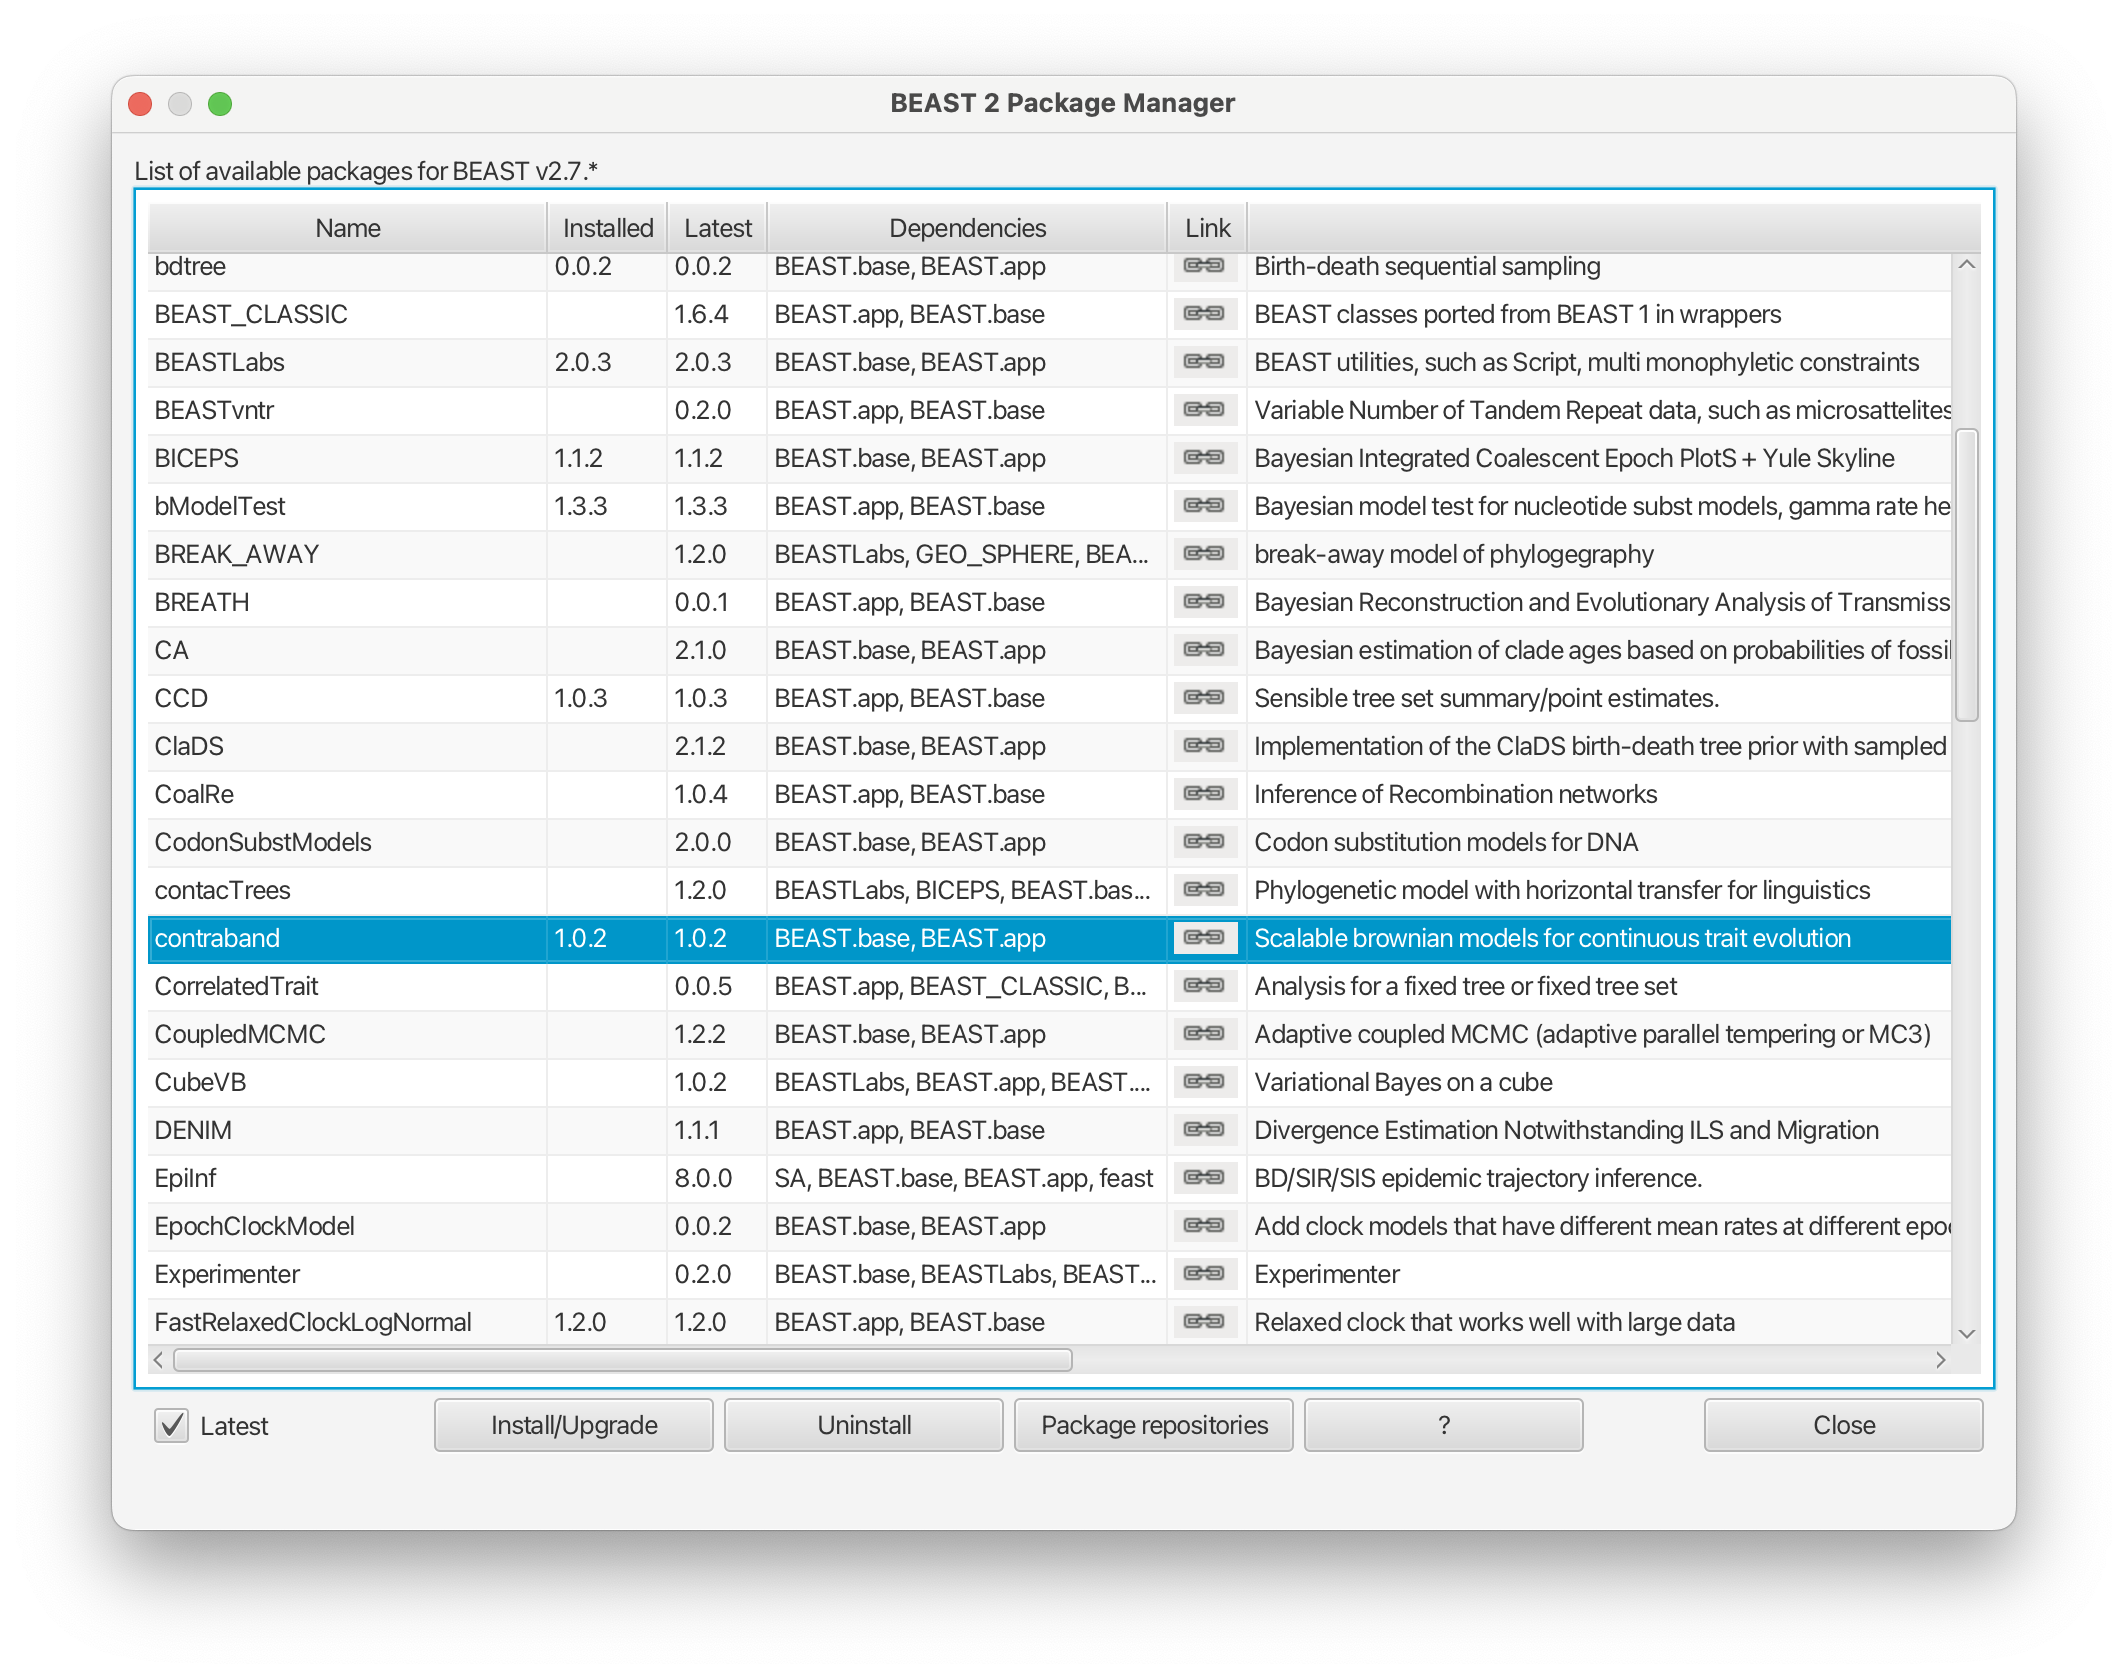
\includegraphics[width=0.5\textwidth]{figures/contrabandDownload.png}
    \caption{Download the contraband package.}
    \label{fig:example1}
\end{figure}

contraband will only be available in BEAUti once you close and restart the
program.

\subsubsection{Loading the Carnivoran Molecular Sequences}\label{loading-the-molecular-sequences}


\subsubsection{Loading \textbf{DATA} the (Partitions)}

The sequences from the \emph{data} folder name \emph{XXX.nexus} can be either drag and dropped into BEAUti or added using BEAUti’s menu system via \emph{File \textgreater{}\textgreater{} Import Alignment}. Once the sequences are added, we need to specify the sampling dates.
%
\subsubsection{Get the sampling times (Tip Dates)}

Open the "Tip Dates" panel and then select the "Use tip dates" checkbox.

The sampling times are encoded in the sequence names.  We can tell BEAUti 
to use these by clicking the \emph{Auto-configure} button. The sampling times 
appear following the third vertical bar "|" in the sequence name. To extract these times, select "split on character", enter "|" (without the quotes) in the text box immediately to the right, and then select "3" from the drop-down box to the right, as shown in the figure below.
%
%\begin{figure}
%    \centering
%    \includegraphics[width=0.700000\textwidth]{figures/TipDates.png}
%    \caption{Guess sampling times.}
%    \label{fig:example1}
%\end{figure}
%
Clicking "Ok" should now populate the table with the sample times extracted from the sequence names: the column \textbf{Date} should now have values between 2000 and 2002 and the column \textbf{Height} should have values from 0 to 2. The heights denote the time difference from a sequence to the most recently sampled sequence. If everything is 
specified correctly, the sequence with Height 0.0 should have Date 2001.9. 
%
\subsubsection{Specify the Brownian motion Model}
%
%Next, we have to specify the site model. For Influenza Hemagluttanin
%sequences as we have here, HKY is the most commonly used model of
%nucleotide evolution. It allows for difference in transversion and
%transition rates. Meaning that changes between bases that are chemically
%closer related (transitions) are allowed to have a different rate than
%changes between bases that chemically more distinct (transversion).
%Additionally, we should allow for different rate categories for
%different sites in the alignment. This can be done by setting the
%\emph{Gamma Category Count} to 4, which is just a value that has
%typically been used. Make sure that estimate is checked next to the
%shape parameter. To reduce the number of parameters we have to estimate,
%we can set Frequencies to Empirical.
%
%\begin{figure}
%    \centering
%    \includegraphics[width=0.700000\textwidth]{figures/SiteModel.png}
%    \caption{Set the site model.}
%    \label{fig:example1}
%\end{figure}
%
\subsubsection{Set the clock model (Clock Model)}
%
%For rapidly evolving viruses, the assumption of a strict molecular clock
%is often made, meaning that the molecular clock is the same on each
%branch of the phylogeny. To decrease the burnin phase, we can set the
%initial value to 0.005.
%
%\begin{figure}
%    \centering
%    \includegraphics[width=0.700000\textwidth]{figures/ClockRate.png}
%    \caption{Set the initial clock rate.}
%    \label{fig:example1}
%\end{figure}
%
\subsubsection{Specify the priors (Priors)}
%
Now, we need to set the priors for the various parameters of the model. 
You can find the parameter priors below the tree prior.
%
%First, consider the effective population size parameter \emph{Ne}. Since we
%have only a few samples per location, meaning little information about the
%different effective population sizes, we will need an informative prior. 
%In this case we will use a log normal prior with parameters M=0 and S=1. 
%(These are respectively the mean and variance of the corresponding normal 
%distribution in log space.) To use this prior, choose "Log Normal" from 
%the drop down menu to the right of the \emph{Ne.t:H3N2} parameter label, 
%then click the arrow to the left of the same label and fill in the parameter 
%values appropriately (i.e. M=0 and S=1). Ensure that the "Mean In Real Space" 
%checkbox remains unchecked.
%
%The existing exponential distribution as a prior on the migration rate puts 
%much weight on lower values while not prohibiting larger ones. For migration 
%rates, a prior that prohibits too large values while not greatly distinguishing between very small and very \textbf{very} small values is generally a good choice. 
%Be aware however that the exponential distribution is quite an informative prior: one should be careful that to choose a mean so that feasible rates are at least within the 95\% HPD interval of the prior.  (This can be determined by clicking the arrow to the left of the parameter name and looking at the values below the graph that appears on the right.) We keep the default mean value of 1.
%
%Finally, set the prior for the clock rate. We have a good idea about the clock 
%rate of Influenza A/H3N2 Hemagglutinin. From previous work by other people, 
%we know that the clock rate will be around 0.005 substitution per site per year. To include that prior knowledge, we can set the prior on the clock rate to a Log Normal distribution with mean in \textbf{real space} set to 0.005. To specify the mean in real space, make sure that the box "Mean In Real Space" is checked. If  we set the S value to 0.25, we say that we expect the clock rate to be with 95\%  certainty between 0.00321 and 0.00731.
%
%\begin{figure}
%    \centering
%    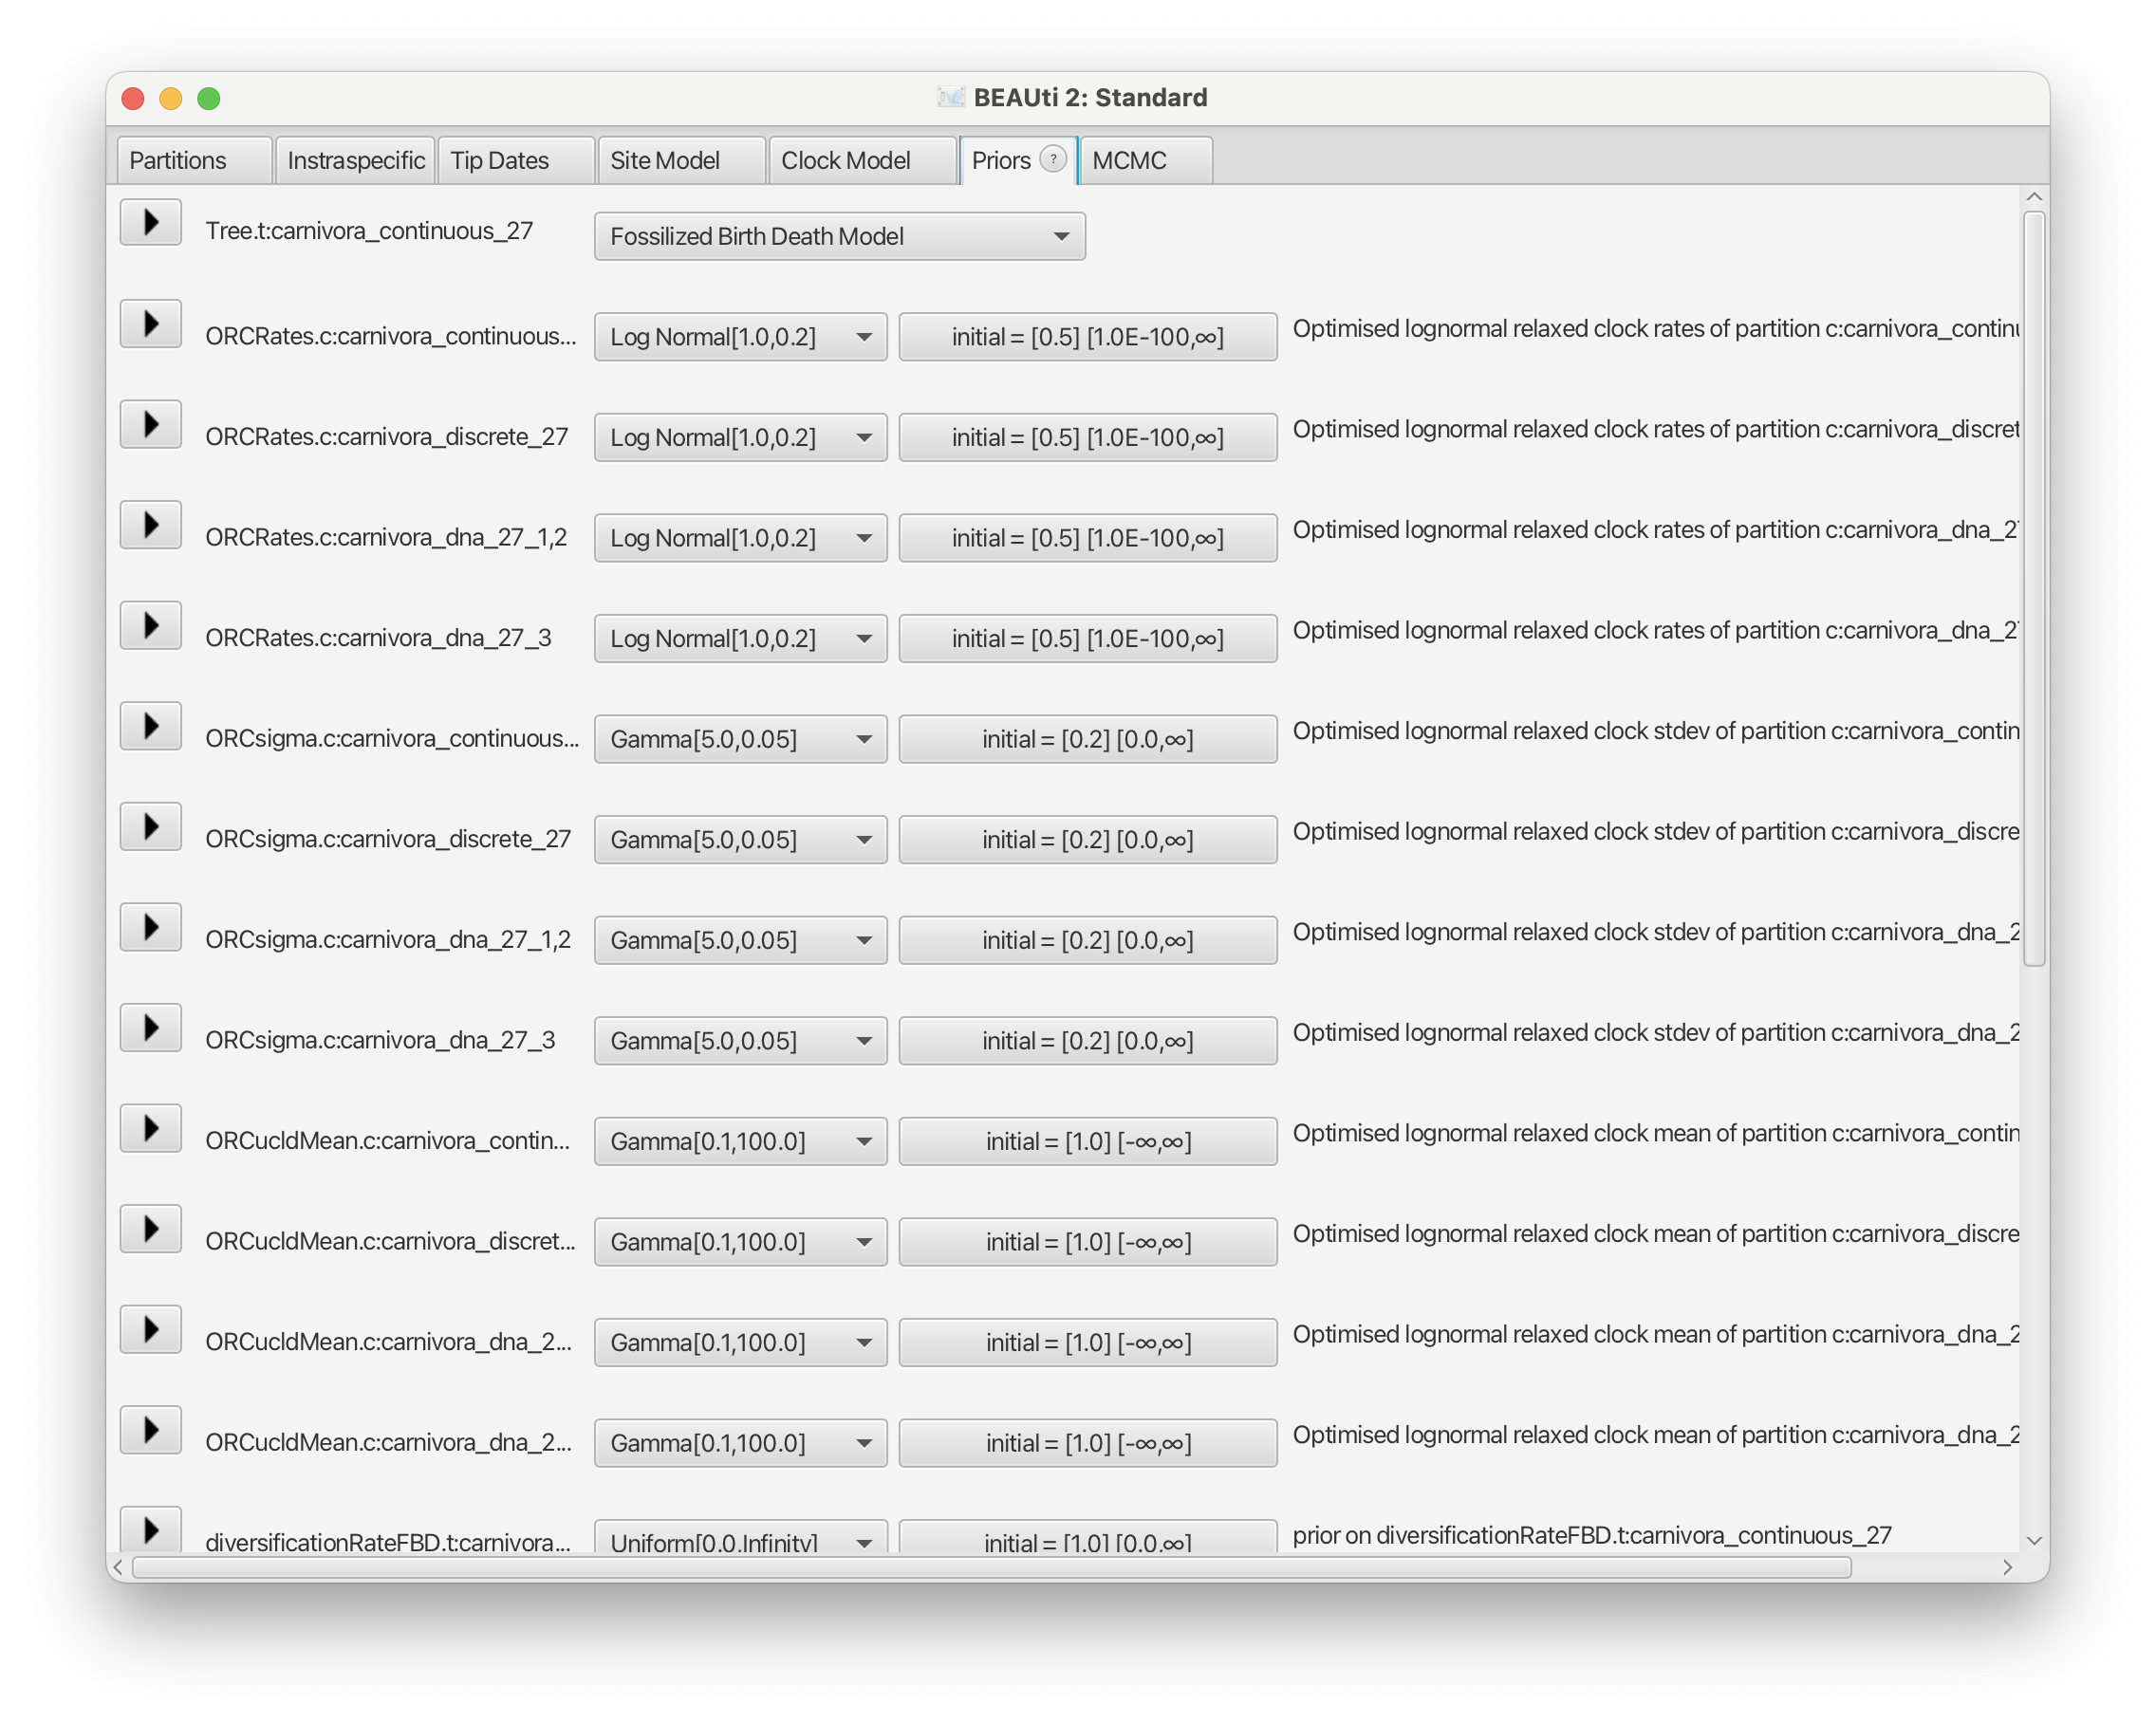
\includegraphics[width=0.700000\textwidth]{figures/Priors.png}
%    \caption{Set up of the prior distributions.}
%    \label{fig:example1}
%\end{figure}
%
%We keep the default priors for the parameters gammaShape and kappa.
%

\subsubsection{Specify the MCMC chain length (MCMC)}\label{specify-the-mcmc-chain-length-mcmc}
%
Here we can set the length of the MCMC chain and after how many
iterations the parameter and trees a logged. For this dataset, 2 million
iterations should be sufficient. In order to have enough samples but not
create too large files, we can set the logEvery to 2000, so we have 1001
samples overall. Next, we have to save the \lstinline!*.xml! file under
\emph{File \textgreater{}\textgreater{} Save as}.
%
%\begin{figure}
%    \centering
%    \includegraphics[width=0.700000\textwidth]{figures/MCMC.png}
%    \caption{save the *.xml.}
%    \label{fig:example1}
%\end{figure}
%
\subsubsection{Run the Analysis using BEAST2}\label{run-the-analysis-using-beast2}
%
Run the \lstinline!*.xml! using BEAST2 or use finished runs from the
\emph{precooked-runs} folder. The analysis should take about 6 to 7
minutes.
%

\section{Practical  Part \uppercase\expandafter{\romannumeral 3}:  Post analysis}

\subsubsection{Analyse the log file using Tracer}\label{analyse-the-log-file-using-tracer}
%
First, we can open the \lstinline!*.log! file in tracer to check if the
MCMC has converged. The ESS value should be above 200 for almost all
values and especially for the posterior estimates. 
%
%\begin{figure}
%    \centering
%    \includegraphics[width=0.700000\textwidth]{figures/LogPosterior.png}
%    \caption{Check if the posterior converged.}
%    \label{fig:example1}
%\end{figure}
%
%Next, we can have a look at the inferred effective population sizes. New
%York is inferred to have the largest effective population size before
%Hong Kong and New Zealand. This tells us that two lineages that are in
%the New Zealand are expected to coalesce quicker than two lineages in
%Hong Kong or New York.
%
%\begin{figure}
%    \centering
%    \includegraphics[width=0.700000\textwidth]{figures/LogNe.png}
%    \caption{Compare the different inferred effective population sizes.}
%    \label{fig:example1}
%\end{figure}
%
%In this example, we have relatively little information about the
%effective population sizes of each location. This can lead to estimates
%that are greatly informed by the prior. Additionally, there can be great
%differences between median and mean estimates. The median estimates are
%generally more reliable since they are less influence by extreme values.
%
%\begin{figure}
%    \centering
%    \includegraphics[width=0.700000\textwidth]{figures/MeanMedian.png}
%    \caption{Differences between Mean and Meadian estimates.}
%    \label{fig:example1}
%\end{figure}
%
%We can then look at the inferred migration rates. The migration rates
%have the label b\_migration.*, meaning that they are backwards in time
%migration rates. The highest rates are from New York to Hong Kong.
%Because they are backwards in time migration rates, this means that
%lineages from New York are inferred to be likely from Hong Kong if we're
%going backwards in time. In the inferred phylogenies, we should
%therefore make the observation that lineages ancestral to samples from
%New York are inferred to be from the Hong Kong backwards.
%
%\begin{figure}
%    \centering
%    \includegraphics[width=0.700000\textwidth]{figures/LogMigration.png}
%    \caption{Compare the inferrred migration rates.}
%    \label{fig:example1}
%\end{figure}

\subsubsection{Make the summary tree using TreeAnnotator}
%
%Next, we want to summarize the trees. This we can do using TreeAnnotator. Until recently the \textit{maximum clade credibility} tree (MCC) has been the default summary method in TreeAnotator. To produce MCC trees TreeAnotator takes the set of trees and find the best supported tree by maximising the product of the posterior clade probabilities. It will then annotate this representative summary tree with the mean ages of all the nodes and the corresponding 95\% HPD ranges as well as the posterior clade probability for each node. A new point estimate, called a \textit{conditional clade distribution} tree (CCD) has been proposed  \citep{berling2025}. It has been shown to outperform MCC in terms of accuracy (based on Robinson-Foulds distance to the true tree) and precision (how different are the point estimates calculated for replicate MCMC chains). CCD methods may produce a tree that would be well supported but has not been sampled during MCMC. This is beneficial for large trees and complex parameter regimes. Since both methods are still widely used, we show how to use them to summarise the posterior tree distribution. \textbf{To save time, you may run just one method and compare it to the other using the example below.}
%
%
\textbf{Producing MCC tree}
%
\begin{framed}
Open \textbf{TreeAnnotator} and then set the options as in the Figure \ref{fig:example1} below. You have to specify the \textbf{Burnin percentage}, \textbf{Target tree type},  \textbf{Node heights}, \textbf{Input Tree File} and the \textbf{Output File}.
Use the typed trees in the file  \lstinline!H3N2.H3N2.trees! as \textbf{Input Tree File}. Name output file \lstinline!H3N2.mcc.tree!.
After clicking \textbf{Run} the program should summarize the trees.
\end{framed}
%
%\begin{figure}
%    \centering
%    \includegraphics[width=0.500000\textwidth]{figures/TreeAnnotator.png}
%    \caption{Make the maximum clade credibility tree.}
%    \label{fig:example1}
%\end{figure}
%
%\textbf{Producing CCD0 tree}
%
%To produce CCD0 summary tree, you will first need to install the CCD package.
%
%\begin{framed}
%	Open BEAUTi and select \textbf{File} >> \textbf{Manage packages}
%	
%	Select \textbf{CCD} package in the list and select \textbf{Install/Upgrade} (see Figure \ref{fig:installCCD})
%	
%	Close BEAUTi
%\end{framed}
%
%\begin{figure}[h]
%	\centering
%	\includegraphics[width=0.600000\textwidth]{figures/installCCD0.png}
%	\caption{Install CCD package.}
%	\label{fig:installCCD}
%\end{figure}
%
%Now you can proceed to make CCD0 tree:
%
%\begin{framed}
%	Open \textbf{TreeAnnotator} and then set the options as in the Figure \ref{fig:ccd0} below. You have to specify the \textbf{Burnin percentage}, \textbf{Target tree type}, \textbf{Node heights}, \textbf{Input Tree File} and the \textbf{Output File}.
%	Use the typed trees in the file  \lstinline!H3N2.H3N2.trees! as \textbf{Input Tree File}. Name output file \lstinline!H3N2.ccd0.tree!.
%	After clicking \textbf{Run} the program should summarize the trees.
%\end{framed}
%
%\begin{figure}
%	\centering
%	\includegraphics[width=0.600000\textwidth]{figures/treeannotator.ccd0.png}
%	\caption{Make the conditional clade credibility tree.}
%	\label{fig:ccd0}
%\end{figure}
%
\subsubsection{Analyse and compare the MCC trees}

\subsubsection{Errors that can occur (Work in progress)}
%
%One of the errors message that can occur regularly is the following:
%\emph{too many iterations, return negative infinity}.
%This occurs when the integration step size of the ODE's to compute the probability of observing a phylogenetic tree in MASCOT is becoming too small.
%This generally occurs if at least one migration rate is really large or at least one effective population size is really small (i.e. the coalescent rate is really high). This causes integration steps to be extremely small, which in turn would require a lot of time to compute the probability of a phylogenetic tree under MASCOT. Instead of doing that, this state is rejected by assigning its log probability the value negative infinity.
%
%This error can have different origins and a likely incomplete list is the following:
%\begin{enumerate}
%\item The priors on migration rates put too much weight on really high rates. To fix this, reconsider your priors on the migration rates. Particularly, check if the prior on the migration rates make sense in comparison to the height of the tree. If, for example, the tree has a height of 1000 years, but the prior on the migration rate is exponential with mean 1, then the prior assumption is that between any two states, we expected approximately
% 1000 migration events.
%\item  The prior on the effective population sizes is too low, meaning that the prior on the coalescent rates (1 over the effective population size) is too high. This can for example occur when the prior on the effective population size was chosen to be 1/X. To fix, reconsider your prior on the effective population size.
%\item  There is substantial changes of the effective population sizes and/or migration rates over time that are not modeled. In that case, changes in the effective population sizes or migration rates have to be explained by population structure, which can again lead to some effective population sizes being very low and some migration rates being very high. In that case, there is unfortunately not much that can be done, since MASCOT is not an appropriate model for the dataset.
%\item  There is strong subpopulation structure within the different subpopulations used. In that case, reconsider if the individual sub-populations used are reasonable.
%\end{enumerate}
%
%
%\section{Useful Links}\label{useful-links}
%
%If you interested in the derivations of the marginal approximation of the structured coalescent, you can find them here \citep{Mueller2017}. This paper also explains the mathematical differences to other methods such as the theory underlying BASTA. To get a better idea of how the states of internal nodes are calculated, have a look in this paper \citep{mueller2017mascot}.
%
%\begin{itemize}
%
%\item
%  MASCOT source code: \url{https://github.com/nicfel/Mascot}
%\item
%  \href{http://www.beast2.org/book.html}{Bayesian Evolutionary Analysis
%  with BEAST 2} \citep{BEAST2book2014}
%\item
%  BEAST 2 website and documentation: \url{http://www.beast2.org/}
%\item
%  Join the BEAST user discussion:
%  \url{http://groups.google.com/group/beast-users} 
%\end{itemize}
%
%



%%%%%%%%%%%%%%%%%%%%%%%
% Tutorial disclaimer %
%%%%%%%%%%%%%%%%%%%%%%%
% Please do not change the license
% Add the author names and relevant links
% Add any other aknowledgments here
%\href{http://creativecommons.org/licenses/by/4.0/}{
\includegraphics[scale=0.8]{figures/ccby.pdf}} This tutorial was written by Nicola F. Müller for \href{https://taming-the-beast.github.io}{Taming the BEAST} and is licensed under a \href{http://creativecommons.org/licenses/by/4.0/}{Creative Commons Attribution 4.0 International License}. 


%%%%%%%%%%%%%%%%%%%%
% Do NOT edit this %
%%%%%%%%%%%%%%%%%%%%
Version dated: \today




%%%%%%%%%%%%%%%%
%  REFERENCES  %
%%%%%%%%%%%%%%%%

\printbibliography[heading=relevref]


\end{document}